\section{Rationalité économique et raisonnements stratégiques}

This chapter closes the «~micro~» half with two pieces of economic reasoning. The
first is rationalité: what it means for a consumer's choices to be compatible with
their préférences, the three axioms those préférences are asked to satisfy, and the
difficulties raised against the third. The préférences révélées then read the
préférences off the choices themselves, and the Weak Axiom of Revealed Preference
(WARP) is the consistency those choices must show.\\

The second is strategic reasoning, where several joueurs choose and the utilité of
each depends on what the others do. A jeu is defined by its joueurs, their actions
and their préférences, and two jeux are given by their tables, the dilemme du
prisonnier and Bach ou Stravinsky. An équilibre de Nash is a profil d'actions from
which no joueur gains by deviating; the chapter gives a method for finding one, the
elimination of the stratégies dominées, and names the fields where it is applied.

\subsection{La rationalité économique}

The notion comes with its advantage stated first: «~Avantage~: concept
mathématique~».

\begin{definition}[Rationalité (\textit{rationality})]
  Rationalité = compatibilité entre les choix/actions et les préférences
  (\textbf{fonction d'utilité} (\textit{utility function}) avec les bonnes
  propriétés)~:
  \begin{itemize}
    \item l'action choisie doit être au moins aussi bonne en termes de préférences
      qu'une autre action disponible~;
    \item $u(x) > u(y)$ si et seulement si $x$ est préféré à $y$.
  \end{itemize}
\end{definition}

The first point is the one the course stresses: a rational agent picks an action
that is, by their préférences, at least as good as any other action available. The
second ties the préférences to the fonction d'utilité $u$: $u$ gives $x$ a higher
value than $y$ exactly when $x$ is préféré to $y$. Only the order of these values
counts.

\begin{prop}
  L'\textbf{ordinalité} (\textit{ordinality}) de la fonction d'utilité suffit~;
  choix compatible avec une transformation croissante de la fonction d'utilité.
\end{prop}

A transformation croissante changes the values of $u$ but keeps their order, so a
choice compatible with $u$ stays compatible with the transformed function.

\begin{notation}
  Préférences compare two bundles, $x = (x_1, x_2)$ and $y = (y_1, y_2)$, and are
  written with three signs.
  \begin{itemize}
    \item Le consommateur \textbf{préfère $x$ à $y$ strictement}
      (\textit{strictly prefers x to y})~: $(x_1, x_2) \succ (y_1, y_2)$~;
    \item le consommateur est \textbf{indifférent entre $x$ et $y$}
      (\textit{indifferent between x and y})~: $(x_1, x_2) \sim (y_1, y_2)$~;
    \item le consommateur \textbf{préfère $x$ à $y$ faiblement}
      (\textit{weakly prefers x to y})~: $(x_1, x_2) \succeq (y_1, y_2)$.
  \end{itemize}
\end{notation}

Each bundle is written by its two components; the figures below plot $x_1$ on the
horizontal axis and $x_2$ on the vertical one. The axioms are stated with the weak
sign $\succeq$.

\begin{definition}[Axiomes]
  Les préférences sont~:
  \begin{itemize}
    \item \emph{complètes}~: pour tout bundle $x$ et $y$,
      $(x_1, x_2) \succeq (y_1, y_2)$ ou $(y_1, y_2) \succeq (x_1, x_2)$ ou les
      deux~;
    \item \emph{réflexives}~: $(x_1, x_2) \succeq (x_1, x_2)$~;
    \item \emph{transitives}~: si $(x_1, x_2) \succeq (y_1, y_2)$ et
      $(y_1, y_2) \succeq (z_1, z_2)$, alors $(x_1, x_2) \succeq (z_1, z_2)$.
  \end{itemize}
\end{definition}

Complete préférences can compare any two bundles; reflexive ones rank each bundle
at least as good as itself; transitive ones let the comparisons chain, through a
third bundle $z = (z_1, z_2)$, from $x$ to $z$.\\

The third axiom is the one put in question: «~Le troisième axiome est
problématique~». Three difficulties are listed with it.

\begin{enumerate}
  \item «~Peut-on classer les trois bundles~? Quatre, cinq, \ldots~?~» The third
    axiom involves three bundles; the question is whether a consumer can rank
    three of them, and then four, five or more.
  \item The \emph{Independence of Irrelevant Alternatives} (IIA)~: «~Si $x$ est
    préféré à $y$, alors ajouter une option $z$ qui n'est pas pertinente n'a pas
    d'effets.~»
  \item The \textbf{biais cognitifs} (\textit{cognitive biases})~:
    «~Manipulations en utilisant les neuro-sciences~», with two cases named, the
    procès Facebook/Meta and the Dark patterns.
\end{enumerate}

The IIA comes with an example, the only one of the three difficulties to be
developed.

\begin{example}[Carte de restaurant]
  «~Carte de restaurant~: $x$ = steak (20~EUR), $y$ = poulet (15~EUR), le
  consommateur préfère $y$ à $x$~; le consommateur est allergique aux fruits de mer
  mais on lui propose une nouvelle carte avec en plus du homard (40~EUR)~; le
  poulet paraît cheap et maintenant le consommateur préfère le plat intermédiaire
  (steak).~»\\

  The homard plays the part of $z$: the consumer is allergic to it, so it is not an
  option they would take. Yet once it is on the menu the poulet looks cheap beside
  it, and the choice between $x$ and $y$ turns round, to the steak, now the dish in
  the middle of the price range. Adding an option that is not relevant has had an
  effect, which IIA rules out.
\end{example}

\subsection{Les préférences révélées}

The \textbf{préférences révélées} (\textit{revealed preference}) read a consumer's
préférences off what they buy, by comparing the bundle they chose with the bundles they
could have bought instead. «~Le bundle $(x_1, x_2)$ est acheté aux prix
$(p_1, p_2)$. Comme $(y_1, y_2)$ est abordable, cela signifie que la contrainte
budgétaire est satisfaite~: $p_1 y_1 + p_2 y_2 \le m$.~» Here $m$ is what the
consumer has to spend, the right-hand side of the contrainte budgétaire.\\

The figure draws the case. The bundles that satisfy the contrainte budgétaire, the
abordable ones, fill the shaded triangle under the line; the chosen bundle
$(x_1, x_2)$ lies on the line, and $(y_1, y_2)$ inside the triangle. The bundle
$(x_1, x_2)$ that the consumer chooses is therefore \textbf{révélé préféré}
(\textit{revealed preferred}) to the bundle $(y_1, y_2)$, a bundle they could have
chosen.

\begin{figure}[h!]
  \centering
  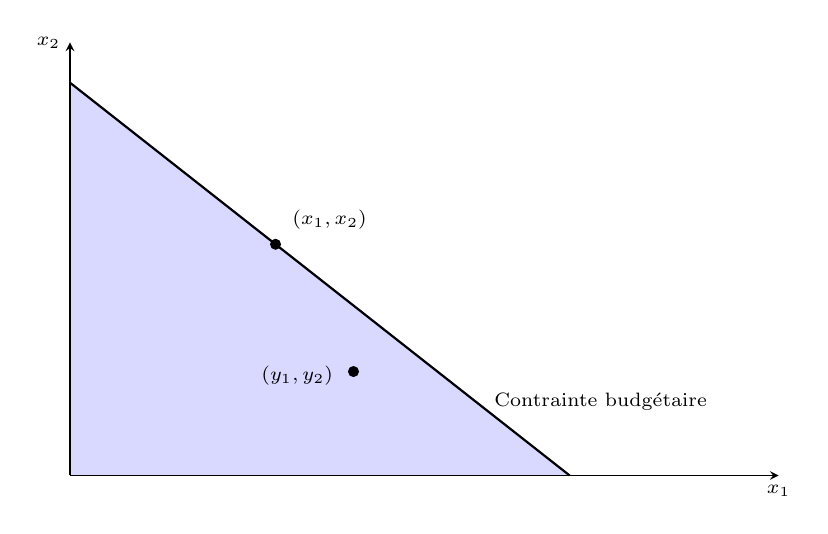
\begin{tikzpicture}[x=0.09cm, y=0.055cm, font=\scriptsize, >=stealth,
      dot/.style={circle, fill=black, inner sep=0pt, minimum size=4pt}]
    \fill[blue!15] (0,0) -- (0,90.7) -- (70.5,0) -- cycle;
    \draw[->] (0,0) -- (100,0) node[below] {$x_1$};
    \draw[->] (0,0) -- (0,100) node[left] {$x_2$};
    \draw[thick] (0,90.7) -- (70.5,0);
    \node[dot] at (29,53.39) {};
    \node[anchor=south west] at (30,54.5) {$(x_1, x_2)$};
    \node[dot] at (40,24) {};
    \node[anchor=east] at (38.5,23) {$(y_1, y_2)$};
    \node[anchor=west] at (58.5,17) {Contrainte budgétaire};
  \end{tikzpicture}
  \caption*{\small Les préférences révélées. The shaded set holds the bundles that
  are abordable at the prices $(p_1, p_2)$. The consumer chooses $(x_1, x_2)$, on
  the contrainte budgétaire, although $(y_1, y_2)$ was abordable: $(x_1, x_2)$ is
  révélé préféré to $(y_1, y_2)$.}
\end{figure}

\subsubsection{Le principe des préférences révélées}

The principle turns that reading into a rule.

\begin{definition}[Principe des préférences révélées (\textit{principle of revealed preference})]
  Si $y$ est abordable (respecte la contrainte budgétaire) aux prix $(p_1, p_2)$ et
  que $x$ est choisi, alors $x$ est révélé préféré à $y$~: soit $(x_1, x_2)$ le bundle
  choisi aux prix $(p_1, p_2)$, soit $(y_1, y_2)$ tel que
  $p_1 x_1 + p_2 x_2 \ge p_1 y_1 + p_2 y_2$, alors $(x_1, x_2) \succeq (y_1, y_2)$.
\end{definition}

That $y$ is abordable when $x$ is chosen is written as a comparison of costs: at these prices, $y$ costs no more than $x$. What
the choice reveals is the weak préférence $\succeq$: $x$ is at least as good as
$y$.

\subsection{Weak Axiom of Revealed Preference}

WARP asks the consumer's choices at different prices to be consistent with one
another.

\begin{definition}[Weak Axiom of Revealed Preference (WARP)]
  Si le bundle $y$ est abordable quand le bundle $x$ est acheté, alors si le
  bundle $y$ est acheté, cela implique que le bundle $x$ n'était pas abordable.\\
  Si $(x_1, x_2)$ est révélé préféré au bundle $(y_1, y_2)$, et ces deux bundles
  ne sont pas les mêmes, alors $(y_1, y_2)$ ne peut pas être révélé préféré à
  $(x_1, x_2)$.
\end{definition}

The two sentences state the same axiom; the second puts it in terms of révélé
préféré and adds that the two bundles differ. If $y$ was abordable when $x$ was
bought, $x$ is révélé préféré to $y$; then $y$ may not be révélé préféré to $x$, so
if $y$ is bought at other prices, $x$ cannot have been abordable at those prices.
Two figures show choices that satisfy WARP and choices that violate it.\\

In the first, $(x_1, x_2)$ is chosen on the steeper contrainte budgétaire and
$(y_1, y_2)$ on the flatter one. Each chosen bundle lies above the other
contrainte budgétaire: when one was bought, the other was not abordable. Neither
is révélé préféré to the other, and these choices satisfy WARP. They are
consistent with possible courbes d'indifférence, such as the two drawn, each
tangent to its contrainte budgétaire at the bundle chosen there.\\

In the second, the bundles have swapped lines: $(x_1, x_2)$ is chosen on the
flatter contrainte budgétaire and $(y_1, y_2)$ on the steeper one, and each lies
below the other contrainte budgétaire. Each was abordable when the other was
bought, so each is révélé préféré to the other: a consumer who chooses both
$(x_1, x_2)$ and $(y_1, y_2)$ violates WARP.

\begin{figure}[h!]
  \centering
  \begin{minipage}[t]{0.48\textwidth}
    \centering
    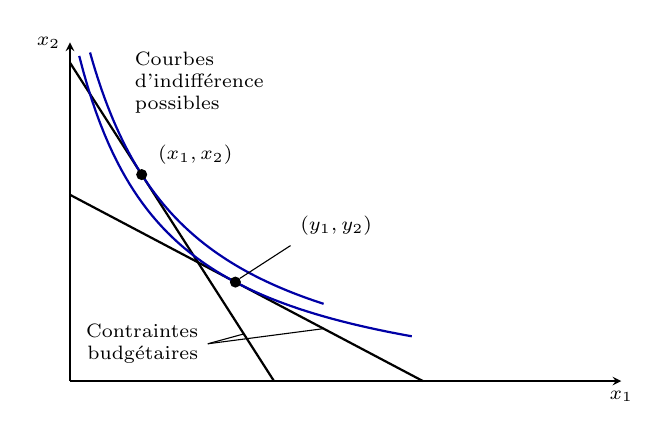
\begin{tikzpicture}[x=0.07cm, y=0.043cm, font=\scriptsize, >=stealth,
        dot/.style={circle, fill=black, inner sep=0pt, minimum size=4pt},
        ic/.style={blue!65!black, thick}]
      \draw[->] (0,0) -- (100,0) node[below] {$x_1$};
      \draw[->] (0,0) -- (0,100) node[left] {$x_2$};
      % two budget lines
      \draw[thick] (0,94) -- (37,0);
      \draw[thick] (0,55) -- (64,0);
      % possible indifference curves: (x - d)(y - e) = k, one tangent at each bundle
      \draw[ic] plot[domain=3.63:46, samples=80]
        (\x, {1932.23/(\x + 14.5782) - 9.0907});
      \draw[ic] plot[domain=1.67:62, samples=80]
        (\x, {1707.77/(\x + 14.5782) - 9.0907});
      \node[anchor=north west, align=left] at (10,100)
        {Courbes\\d'indifférence\\possibles};
      % chosen bundles
      \node[dot] at (13,60.97) {};
      \node[anchor=south west] at (14.2,61) {$(x_1, x_2)$};
      \node[dot] at (30,29.22) {};
      \node[anchor=south west] (y) at (40,40) {$(y_1, y_2)$};
      \draw (y.south west) -- (30.8,30.3);
      % label of the budget lines
      \node[anchor=east, align=right] (b) at (25,11) {Contraintes\\budgétaires};
      \draw (b.east) -- (31.5,13.9);
      \draw (b.east) -- (46,15.47);
    \end{tikzpicture}
    \caption*{\small WARP vérifié. Each chosen bundle lies above the other
    contrainte budgétaire, so neither was abordable when the other was bought; the
    choices satisfy WARP and are consistent with courbes d'indifférence such as
    these, each tangent to its contrainte budgétaire at the bundle chosen.}
  \end{minipage}
  \hfill
  \begin{minipage}[t]{0.48\textwidth}
    \centering
    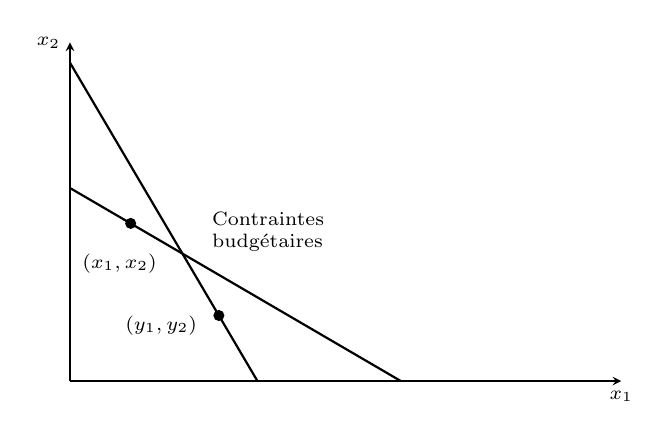
\begin{tikzpicture}[x=0.07cm, y=0.043cm, font=\scriptsize, >=stealth,
        dot/.style={circle, fill=black, inner sep=0pt, minimum size=4pt}]
      \draw[->] (0,0) -- (100,0) node[below] {$x_1$};
      \draw[->] (0,0) -- (0,100) node[left] {$x_2$};
      % two budget lines
      \draw[thick] (0,94) -- (34,0);
      \draw[thick] (0,57) -- (60,0);
      \node[anchor=west, align=left] at (24,44) {Contraintes\\budgétaires};
      % chosen bundles
      \node[dot] at (11,46.55) {};
      \node[anchor=north] at (9,40.5) {$(x_1, x_2)$};
      \node[dot] at (27,19.35) {};
      \node[anchor=east] at (24.8,16.5) {$(y_1, y_2)$};
    \end{tikzpicture}
    \caption*{\small WARP non vérifié. Each chosen bundle lies below the other
    contrainte budgétaire, so each was abordable when the other was bought: a
    consumer who chooses both $(x_1, x_2)$ and $(y_1, y_2)$ violates WARP.}
  \end{minipage}
\end{figure}

\subsection{Jeux stratégiques}

The \textbf{jeux stratégiques} (\textit{strategic games}) take the choice from one
agent to several.

\begin{definition}[Jeu (\textit{game})]
  Un jeu consiste en~:
  \begin{itemize}
    \item un ensemble de \textbf{joueurs} (\textit{players})~;
    \item pour chaque joueur, un ensemble d'actions~;
    \item pour chaque joueur, des préférences sur les profils d'actions possibles.
  \end{itemize}
\end{definition}

Each profil d'actions, defined with the équilibre de Nash below, holds one action
per joueur, so the utilité $u_i$ of joueur $i$ depends on what the others do, not on
their own action alone.\\

Under «~Timing~», the actions are \textbf{actions successives} (\textit{sequential
moves}) or \textbf{actions simultanées} (\textit{simultaneous moves}), and
«~cela dépend des informations~».

\subsubsection{Le dilemme du prisonnier}

The first jeu, the \textbf{dilemme du prisonnier} (\textit{prisoner's dilemma}),
is given by its table alone. Its two joueurs are Suspect~1, who chooses the row,
and Suspect~2, who chooses the column; each can se taire or dénoncer the other, and
each cell gives the utilité of Suspect~1, then that of Suspect~2.

\begin{center}
  \small
  \begin{tabular}{@{}llcc@{}}
    \toprule
    & & \multicolumn{2}{c}{Suspect 2} \\
    \cmidrule(l){3-4}
    & & Se taire & Dénoncer \\
    \midrule
    \multirow{2}{*}{Suspect 1} & Se taire & $(2, 2)$ & $(0, 3)$ \\
                               & Dénoncer & $(3, 0)$ & $(1, 1)$ \\
    \bottomrule
  \end{tabular}
\end{center}

\subsection{L'équilibre de Nash}

Three points come with the \textbf{équilibre de Nash} (\textit{Nash equilibrium}):
\begin{itemize}
  \item les joueurs sont rationnels~;
  \item connaissance commune~;
  \item aucun des joueurs n'a intérêt à dévier (pas de \textbf{déviation
    profitable} (\textit{profitable deviation})).
\end{itemize}
The connaissance commune is only named. The definition writes the third point with
the utilités $u_i$.

\begin{definition}[Équilibre de Nash]
  Soit $a$ un \textbf{profil d'actions} (\textit{action profile}), avec $a_i$
  l'action du joueur $i$ et $a_{-i}$ les actions des autres joueurs. Un profil
  d'actions peut être écrit $a = (a_i, a_{-i})$.\\
  Équilibre de Nash~: aucun joueur ne préfère $(a_i, a^*_{-i})$ à $a^*$. Pour tout
  joueur $i$ et toute action $a_i$ du joueur $i$~:
  \[ u_i(a^*) \ge u_i(a_i, a^*_{-i}). \]
\end{definition}

Here $a^*$ is the profil d'actions of the équilibre de Nash and $a^*_{-i}$ the actions the other
joueurs take in it. With those held fixed, no action $a_i$ gives joueur $i$ a higher
utilité than their action in $a^*$: no joueur has a déviation profitable.

\subsubsection{Bach ou Stravinsky}

The second jeu is also given by its table alone. Each of its two joueurs chooses
Bach or Stravinsky, the first the row and the second the column, and each cell
gives the utilité of the first joueur, then that of the second.

\begin{center}
  \small
  \begin{tabular}{@{}lcc@{}}
    \toprule
    & Bach & Stravinsky \\
    \midrule
    Bach       & $(2, 1)$ & $(0, 0)$ \\
    Stravinsky & $(0, 0)$ & $(1, 2)$ \\
    \bottomrule
  \end{tabular}
\end{center}

\subsubsection{Trouver l'équilibre de Nash}

To find an équilibre de Nash, «~on élimine les \textbf{stratégies dominées}
(\textit{dominated strategies})~». What is defined below is when some actions of a
joueur dominent strictement others; the stratégies dominantes are only named. The
method speaks of stratégies and the definition of actions: they
are the same objects here.

\begin{definition}[Stratégies dominées]
  Les actions $a''_i$ du joueur $i$ \textbf{dominent strictement}
  (\textit{strictly dominate}) les actions $a'_i$ si
  $u_i(a''_i, a_{-i}) > u_i(a'_i, a_{-i})$ pour tout $a_{-i}$.
\end{definition}

Whatever the other joueurs do, $a''_i$ gives joueur $i$ a strictly higher utilité
than $a'_i$. The action $a'_i$ is then a stratégie dominée, the kind of action the
method eliminates.

\subsubsection{Nombreuses applications}

The équilibre de Nash has «~nombreuses applications~». They are named here without
being developed, and the list is left open:
\begin{itemize}
  \item concurrence à la Cournot~;
  \item concurrence à la Bertrand~;
  \item choix de programme politique~;
  \item enchères~;
  \item \ldots
\end{itemize}
